\scanpage{10}

% 1, title
\uline{\deleted{Complexes}\inserted{Cartes} coniques}, \uline{\deleted{complexes}\inserted{cartes} \deleted{cellulaires}}, et \uline{ens. à opérateurs}.

% 2–5, filtered space
Une \uline{$n$-carte conique} \inserted{(finie)} est un espace top. $X$ compact, muni d'une filtration croissante \inserted{par des parties \uline{fermées}}
\[
 X_0\subset X_1\subset\ldots\subset X_{n-1}\subset X_n=X
\]
telles que

% 6, first condition
a) $X_0$ fini (i.e. discret)

% 7–12, second condition
b) pour $1\leq i\leq n$, \inserted{soit $\bar Z_i={}$} $\operatorname{Déc}(X_i/X_{i-1})\deleted{=\bar Z_i}$ (découpage de $X_i$ suivant $X_{i-1}$), $\dot Z_i=\bar Z_i\mid X_{i-1}$ (NB on a $Z_i\to X_i$, induisant un isom. $\bar Z_i-\dot Z_i\longrightarrow X_i-X_{i-1}$), alors \deleted{les composantes} \inserted{$\bar Z_i$ a un n\textsuperscript{b} \uline{fini} de comp. connexes,} et chacune $\bar Z_i^\alpha$ est \unsure{isom.|hom.|homéom.} au cône sur $\dot Z_i^\alpha=\bar Z_i^\alpha\cap\dot Z_i$ (et $\dot Z_i^\alpha\ne\varnothing$)

% 13, finite morphism
c) $\dot Z_i\to X_{i-1}$ est un morphisme fini, \deleted{dont l'image}

% 14, fourth condition and interline
\deleted{\unsure{c)}} d) La filtration de $X$ est équisingulière \inserted{[$\Leftrightarrow\bar Z_i\to X_{\unsure{j|i}-1}$ est \unsure{constant|constante} sur \unsure{les|une} \unsure{comp.|c.c.} de $X_j-X_{j-1}$ $(j\leq i-1)$]}

% 14–16, right of examples
\margin{d) \unsure{Soit|Soit l'} image \inserted{$X'_{i-1}$} de $\bar Z_i$ ds $X_{i-1}$ \deleted{\unsure{$X'_i$}} Alors $X'_{i-1}=\overline{X'_{i-1}\cap\complement X_{i-2}}$}

% 15–16, small dimensions
Cas $n=0$ : espaces finis discrets

Cas $n=1$ : \qquad $\underbrace{X=X_1}_{\text{cpt}}\supset X_0$.

% lower left, decomposition in dimension one
\diagram{\begin{tikzcd}[ampersand replacement=\&,row sep=small,column sep=tiny]
\dot Z_1\arrow[d]\&{}=\coprod_\alpha\dot Z_1^\alpha\\
X_0
\end{tikzcd}}

% lower right, dimensions zero to three
\diagram{\begin{tikzcd}[ampersand replacement=\&,row sep=small,column sep=1ex]
\overset{\deleted{\unsure{x}}}{\dot x_0}\in\overset{\deleted{\unsure{x}}}{y_1}\&\&\overset{\deleted{\unsure{x}}}{\dot x_1}\quad y_2\\
\dot Z_1\arrow[d]\arrow[r,phantom,"\subset" description]\&\overset{\deleted{\unsure{m}}}{\bar Z_1}\arrow[d]\&\dot Z_2\arrow[dl]\arrow[r,phantom,"\subset" description]\&\bar Z_2\arrow[d]\&\dot Z_3\arrow[dl]\arrow[r,phantom,"\subset" description]\&\bar Z_3\arrow[d]\\
 X_0\arrow[r,phantom,"\subset" description]\&X_1\arrow[rr,phantom,"\subset" description]\&\&X_2\arrow[rr,phantom,"\subset" description]\&\&X_3\\
 x_0\arrow[r,phantom,"\subset" description]\&x_1\arrow[rr,phantom,"\subset" description]\&\&x_2\arrow[rr,phantom,"\subset" description]\&\&x_3
\end{tikzcd}}

% lower left, loop with a point
\figure{
\begin{tikzpicture}[scale=.65]\draw (0,0)..controls (.2,.8) and (1.2,1.15)..(1.44,.66)..controls (1.55,.33) and (.45,-.16)..(0,0);\fill (0,0) circle (.055);\end{tikzpicture}}

% lower left, sloping interval
\figure{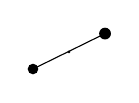
\begin{tikzpicture}[scale=.75]\draw (0,0)--(1.22,.6);\fill (0,0) circle (.09) (.61,.29) circle (.025) (1.22,.6) circle (.1);\end{tikzpicture}}

% lower left, nearly horizontal interval
\figure{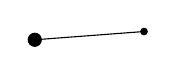
\begin{tikzpicture}[scale=.75]\draw (0,0)--(1.85,.14);\fill (0,0) circle (.12) (1.85,.14) circle (.065);\end{tikzpicture}}

% lower right, general ranks
\diagram{\begin{tikzcd}[ampersand replacement=\&,row sep=small,column sep=1ex]
\dot x_{i+1}\&\dot Z_{i+1}\arrow[d]\arrow[r,phantom,"\subset" description]\& Z_{i+1}\arrow[d,dash]\&\dot Z_{i+2}\arrow[dl]\arrow[r,phantom,"\subset" description]\&\bar Z_{i+2}\arrow[d]\\
X_{i-1}\arrow[r,phantom,"\subset" description]\&X_i\arrow[r,phantom,"\subset" description]\& X_{i+1}\arrow[rr,phantom,"\subset" description]\&\&X_{i+2}\\
\&x_i\&\&\&x_{i+2}
\end{tikzcd}}

% lower left, three branches
\figure{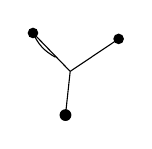
\begin{tikzpicture}[scale=.75]\draw (-.63,.65)--(0,0)--(.82,.55) (0,0)--(-.08,-.74); \draw (-.63,.65) to[bend right=18](-.25,.24); \fill (-.63,.65) circle(.09) (.82,.55) circle(.09) (-.08,-.74) circle(.1);\end{tikzpicture}}

% beside three branches, short stroke
\figure{
\begin{tikzpicture}[scale=.7]\draw[line width=1.2pt](0,0)--(.45,.47);\fill(.45,.47)circle(.055);\end{tikzpicture}}

% bottom left, curved arcs
\figure{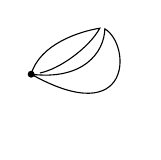
\begin{tikzpicture}[scale=.8]\draw (0,0)..controls (.14,.48) and (.77,.68)..(1.09,.73)..controls (.92,.42) and (.45,.08)..(.14,.02); \draw (0,0)..controls (.82,-.1) and (1.16,.34)..(1.17,.72)..controls (1.59,.47) and (1.61,-.9)..(0,0);\fill (0,0)circle(.055);\end{tikzpicture}}

% bottom middle, sector and rays
\figure{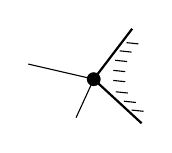
\begin{tikzpicture}[scale=.8]\draw[thick](.61,.8)--(0,0)--(.76,-.7); \draw (-1.04,.24)--(0,0)--(-.28,-.61); \fill(0,0)circle(.11); \foreach \x/\y in {.52/.58,.41/.45,.34/.3,.31/.14,.31/-.02,.35/-.2,.48/-.35,.6/-.49}{\draw (\x,\y)--++(.19,-.02);}\end{tikzpicture}}

% bottom right, restricted terms
\diagram{\begin{tikzcd}[ampersand replacement=\&,row sep=small,column sep=small]
{\dot Z_{i+2}|X_{i-1}}\arrow[d,dash]\arrow[r,phantom,"\subset" description]\&{\dot Z_{i+2}|X_i}\arrow[d]\arrow[r,dash]\&\bar Z_{i+2}\arrow[d]\\
X_{i-1}\arrow[r,phantom,"\subset" description]\&X_i\arrow[r,phantom,"\subset" description]\&X_{i+2}
\end{tikzcd}}

% bottom left, dimension-one square
\diagram{\begin{tikzcd}[ampersand replacement=\&,row sep=tiny,column sep=small]
\dot Z_1\arrow[d]\arrow[r,phantom,"\subset" description]\&\bar Z_1\arrow[d]\\
X_0\arrow[r,phantom,"\subset" description]\&X_1
\end{tikzcd}}

% lower left
% archive sheet number: 9
